\documentclass[12pt]{article}
\usepackage{parskip}
\usepackage[utf8]{inputenc}
\usepackage[T1]{fontenc}
\usepackage{enumitem}
\usepackage{hyperref}
\usepackage{xcolor}
\usepackage{listings}
\usepackage{graphicx}
\usepackage{geometry}

\geometry{a4paper, margin=3cm}

\graphicspath{ {../docs/} }

% \textwidth=16cm

% Hyperlink setup
\definecolor{linkcolor}{rgb}{0,0.4,0.7}
\hypersetup{
    colorlinks=true,
    linkcolor=linkcolor,
    filecolor=magenta,
    urlcolor=linkcolor,
}

% Code block setup
\definecolor{codebg}{rgb}{0.95,0.95,0.95}
\lstset{
    basicstyle=\ttfamily,
    backgroundcolor=\color{codebg},
    breaklines=true,
    frame=single,
}

\title{Eric body language in chat}
\author{Quenten Schoonderwoerd}
\date{\today}

\begin{document}
\maketitle

\section{Inleiding}

Eric zit in een elektrische rolstoel en heeft weinig aan zijn handen.
Hij wil beter lichaamstaal kunnen uiten in chat apps zoals Signal.

\textbf{Opdracht:}
Maak een interface voor hem waarmee hij dit kan bereiken.

\section{Vooronderzoek}

Belangrijk om te begrijpen voordat we verder gaan is hoe we lichaamstaal definieren.
Onder lichaamstaal vallen onder andere dingen zoals: gezichtsexpressie, beweging, postuur en houding van het lichaam.
Er zijn meer dingen die vallen onder dit begrip, maar het is belangrijk voor iedereen om het juiste idee te hebben wanneer we het hebben over lichaamstaal voordat we verdergaan.

Ik heb onderzoeken gelezen over kinesics (lichaamstaal) op het internet.
Er zijn hier namelijk verschillende onderzoeken over geweest.
Zonder hier veel op in te gaan tonen deze onderzoeken voornamelijk aan dat het versturen van lichaamstaal over het internet vrij lastig is.
Er zijn geen echte manieren om non-verbale uitingen zoals lichaamshouding, postuur en houding over te brengen zonder elkaar in persoon te zien.
Zelfs video-communicatie doet hier te weinig voor, omdat het zien van een persoon op een scherm anders aanvoelt dan een echt persoon.

Mijn korte onderzoek laat mij dus denken dat de opdracht zoals direct geinterpreteerd niet mogelijk is om uit te voeren.
Daarom zal moeten worden gekeken naar alternatieven die ook voldoen als antwoord.
Gelukkig bestaan er al methoden om ten minste emotie door te brengen over het internet, voornamelijk met behulp van emoticons.
Andere technieken zijn bijvoorbeeld: stickers, foto's en gifs.

\clearpage\section{Ideeën}
Ik heb in een groep met twee anderen gewerkt aan deze opdracht, namelijk Melvin en Jesse.
Samen hebben wij voorafgaand aan het eerste testmoment een paar ideeën bedacht die we konden uitwerken zodat we iets konden testen op het eerste testmoment.

\begin{enumerate}
	\item Een snelle en efficiente manier om emoji's te zoeken/vinden in een emoticonselectiescherm.
	\item Automatische suggesties van emoji's tijdens het typen.
	\item Emoji's genereren met AI beeldherkenning en afbeelding generatie.
	\item Emoji's suggereren op basis van AI beeldherkenning en emotie analyse.
\end{enumerate}

\subsection{Emoji zoeker}

Dit idee stamt uit een onderzoek dat ik had gelezen dat deelnemers vroeg om bepaalde emoji's te vinden in een standaard emojiselectiescherm, waaruit bleek dat er veel te veel emoji's zijn om snel te vinden wat je zoekt.
Het onderzoek benoemde ook een paar alternatieve methoden waarmee emoji's konden worden gecategoriseerd.

Hieruit hadden wij bedacht dat het eventueel mogelijk kon zijn om op basis van kleur emoji's te groeperen.
Zo zou je op een blauwe knop kunnen drukken en alle emoji's die voornamelijk blauw zijn werden dan beschikbaar.

Een andere manier kan zijn om emoji's te groeperen door middel van emotie, maar dit is veel te subjectief en werkt niet in elke situatie.
Sommige emoji's hebben namelijk andere betekenissen op basis van de context.

\subsection{Emoji suggesties}

Dit idee stamt uit hetzelfde onderzoek als hierboven benoemt, waaruit bleek dat mensen soms moeite hebben met het vinden van de juiste emoji.
Wij bedachten een manier waarmee tekst kon worden geanalyseerd en emoji's konden worden gesuggereerd op basis van deze tekst.

\subsection{Emoji's genereren door beeldherkenning}

Met recente ontwikkelingen op het gebied van AI is het mogelijk om afbeeldingen te genereren met een tekst prompt en zelfs met een andere afbeelding.
Wij bedachten een manier waarmee emoji's door middel van AI konden worden gegenereerd speciaal voor de situatie waar Eric zich op dat moment in bevindt.

\subsection{Emoji's suggereren op basis van AI beeldherkenning en emotie analyse}

Eric zou een foto kunnen nemen van zichzelf wanneer hij via chat emotie wilt doorgeven.
Deze foto zou vervolgens worden geanalyseerd door AI en emoji's kunnen dan worden gesuggereert.
Dit is anders dan het idee hierboven in dat het geen afbeelding generatie bevat, enkel suggesties van al bestaande emoji's.

\clearpage\section{Eerste prototype}

Wij hebben uiteindelijk gekozen om voor de emoji suggesties door middel van tekst te gaan.
Dit idee hebben wij uitgewerkt in een prototype dat we hebben voorgelegd aan Eric, die dit vrij gemakkelijk leek te kunnen gebruiken.

\def\figureautorefname{figuur}
In \autoref{fig:eerste_prototype} is een schermafbeelding te zien van dit prototype.
Wanneer de gebruiker typt in de tekstbalk onderaan het scherm wordt deze tekst doorgestuurd naar een zelf-geschreven API die met behulp van de GPT-3.5 API emoji's suggereert voor deze tekst.
Dit prototype is volledig werkend en op dit moment te vinden op \href{https://eric.ikbenmel.vin}{eric.ikbenmel.vin}.

% Photo of the prototype
\begin{figure}[h]
	\centering
	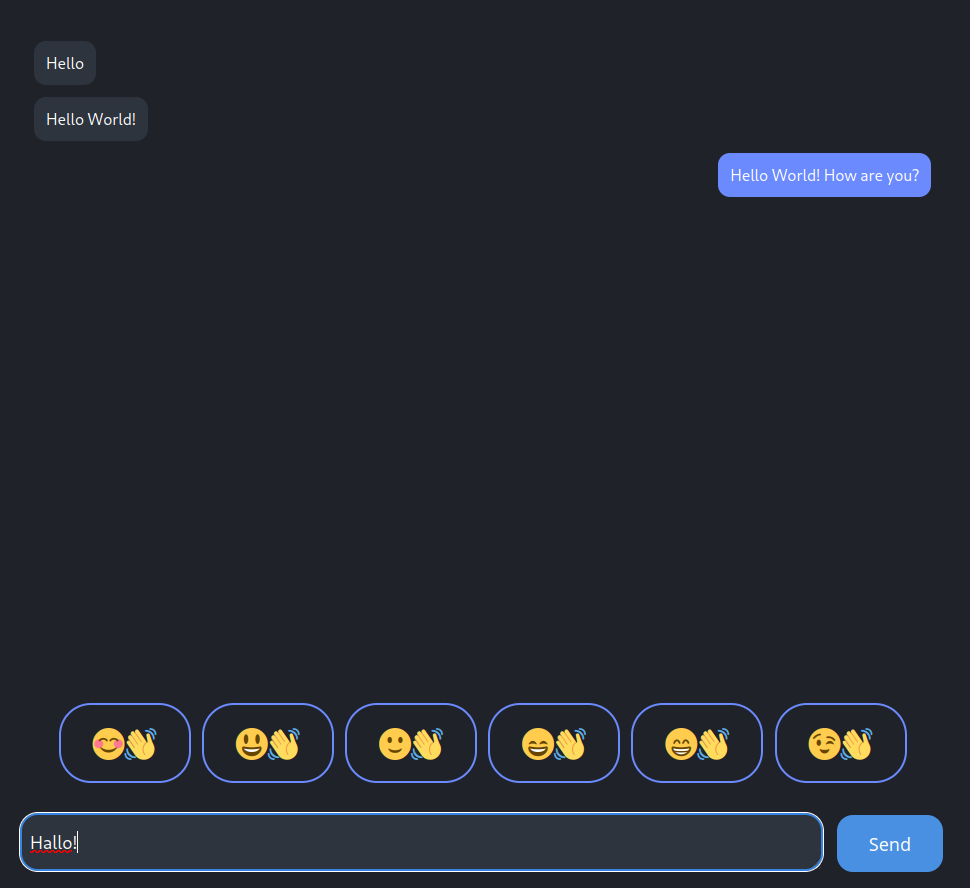
\includegraphics[width=1\textwidth]{eerste_prototype_1}
	\caption{Schermafbeelding van het prototype}
	\label{fig:eerste_prototype}
\end{figure}

De werking van dit prototype op een normale gebruiker is niet super goed totdat de gebruiker doorheeft wat er gebeurt.
Wij hebben dit naast Eric ook op medestudenten getest, die de neiging hadden om direct het bericht te versturen zonder te wachten op de emoji suggesties.
Dit kan komen omdat wij niet vertelde wat het punt was van de app, maar waarschijnlijk speelt de laadtijd ook een grote rol.

Uiteindelijk is de belangrijke test natuurlijk met Eric.

\section{Test \#1 met Eric}

Op 20 April was onze eerste test waarbij we met Eric konden zitten om ons prototype te testen.
Het is ook belangrijk om te zeggen dat dit prototype in ongeveer twee uurtjes in elkaar is gezet en wij nog niet eerder een test hadden gedaan met Eric.
Naast een testsessie was dit ook een belangrijk moment om verder te vragen over Eric's probleem.
Eerst zal ik ingaan op de dingen die wij hebben ondervonden over de opdracht en daarna zal ik verdergaan over de dingen die wij hebben gemerkt tijdens het testen.

\subsection{Achtergrond}

Eric heeft een aandoening waarbij zijn pezen en spieren tijdens niet goed zijn gegroeit.
Dit zorgde ervoor dat zijn ledenmaten anders zijn gegroeit en ontwikkeld dan normaal.
Hij heeft heel weinig controle over zijn vingers en zijn handen zijn ook ingegroeit.

Na het vragen hoe hij zijn telefoon gebruikt en een demonstratie te hebben gekregen konden wij een aantal dingen zien.

Wij wilden voornamelijk weten welk deel van het scherm hij het makkelijkst kan bereiken en welk gebied moeilijk te bereiken is.
Het blijkt dus dat het voor hem helemaal geen probleem is om het hele scherm te bereiken, maar er zijn wel posities waarin zijn hand het scherm bedekt en het scherm voor hem niet meer zichtbaar is.
Typen gaat vrij snel en lijkt geen probleem te zijn, hoewel het corrigeren wel een taak is.

Wij hebben ook gezien hoe hij een selfie maakt.
Dit is een hele klus, omdat hij niet gemakkelijk zijn telefoon kan oppakken en als dat eenmaal is gelukt kan hij niet op het scherm drukken terwijl hij de camera naar hemzelf richt.
Hiervoor gebruikt hij de timer-functie in de camera-app zodat hij op de knop kan drukken en daarna de camera kan richten zoals hij wil.
Dit is een heel gedoe en kost een hoop tijd.
Wij hebben daarom gekozen om de ideeën die een camera vereisen te laten vallen.

Tijdens het gesprek kwamen wij ook meer te weten over de opdracht zelf.
Het schijnt voor hem een frustratiepunt te zijn om emoji's te selecteren, want er zijn er zo veel.
Dit is precies wat ik ook in het vooronderzoek had gelezen.
Hij heeft dus moeite met het vinden van emoji's in het standaard emojiselectiescherm.
Ons prototype waarmee we een emoji suggestie functie hebben gemaakt kwam dus goed aan.

\subsection{Testen}

Voor de test hebben wij ons product laten zien aan Eric en hij heeft het kunnen uitproberen.
Tijdens het typen van de tekst werden er emoji's gesuggereerd die passen bij de tekst.
Het een van de dingen lastig was was om de gebruiker te laten weten hoe het werkt op de eerste keer dat hij het gebruikt.
Een soort tutorial is wel nodig.

Ook is er het probleem dat Eric slecht werkt met zijn handen, dus het is vervelend om een muis te gebruiken.
Een touchscreen gaat wel goed, maar voor een laptop is het gebruik van een muis wel vervelend.
Echter, dit is voor nu wel een acceptabele tekortkoming.





% \section{Lists}
% \subsection{Bullet Points}
% \begin{itemize}
%   \item First item
%   \item Second item
%   \item Third item
% \end{itemize}

% \subsection{Numbered List}
% \begin{enumerate}
%   \item First item
%   \item Second item
%   \item Third item
% \end{enumerate}

% \section{Hyperlinks}
% Here's a link to \href{https://www.example.com}{example.com}.

% \section{Code Blocks}
% Here's a code block:
% \begin{lstlisting}[language=Python]
% def hello_world():
%     print("Hello, World!")

% hello_world()
% \end{lstlisting}

\end{document}
